\section{Maquina de Turing}
	\subsection{Descripción del problema}
	Para este programa se desarrollo una maquina de Turing que acepte el lenguaje $ \left\lbrace 0^{n}1^{n} \mid n\geq 1\right\rbrace  $. Que de manera formal se define como lo siguiente:
	\[ M= ({q_{0}, q_{1}, q_{2}, q_{3}}, q_{4}, {0, 1}, {0, 1, X, Y, B}, \delta, q_{0}, B, {q_{4}}) \]
	donde $\delta$ se especifica como en la siguiente tabla:
	\\
	\begin{center}
		\begin{tabular}{|c|c|c|c|c|c|}
			\hline 
			\multicolumn{6}{|c|}{Símbolo} \\ 
			\hline 
			Estado & 0 & 1 & X & Y & B \\ 
			\hline 
			$q_{0}$ & $(q_{0}, X, R)$ & - & - & $(q_{0}, X, R)$ & - \\ 
			\hline 
			$q_{1}$ & $(q_{0}, X, R)$ & $(q_{0}, X, R)$ & - & $(q_{0}, X, R)$ & - \\ 
			\hline 
			$q_{2}$ & $(q_{0}, X, R)$ & - & $(q_{0}, X, R)$ & $(q_{0}, X, R)$ & - \\ 
			\hline 
			$q_{3}$ & - & - & - & $(q_{0}, X, R)$ & $(q_{0}, X, R)$ \\ 
			\hline 
			$q_{4}$ & - & - & - & - & - \\ 
			\hline 
		\end{tabular}
	\end{center}
	El funcionamiento de esta maquina se puede entender mejor con el diagrama de la figura \ref{fig:turing-diagrama}.
	\begin{figure}[H]
		\begin{center}
			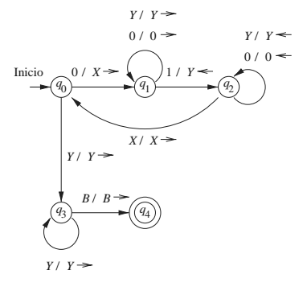
\includegraphics[width=9cm, height=7cm]{img/maquina-diagrama.png}
			\caption{Diagrama de transiciones de una Maquina de Turing que acepta las cadenas $0^{n}1^{n}$. \cite{LIBRO}}
			\label{fig:turing-diagrama}
		\end{center}
	\end{figure}
	El programa debe de contar con un modo manual y automático, en ambos modos se ingresara una cadena de ceros y unos que sera trabajada por la maquina de Turing a través de una unidad de control y una banda (véase la figura \ref{fig:turing}) la cual sera la cadena que se ingrese y se mostrara si es una cadena valida junto al proceso que se realizo para llegar a dicho resultado.
	\begin{figure}[H]
		\begin{center}
		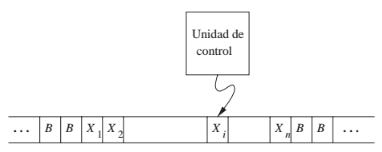
\includegraphics[width=14cm, height=5cm]{img/maquina.png}
		\caption{Representación de una Maquina de Turing. \cite{LIBRO}}
		\label{fig:turing}
		\end{center}
	\end{figure}
	\subsection{Código}
	El código fue realizado en Python 3.5.
	\\Archivo: main\_turing.py
	\begin{lstlisting}[language=Python]
	# main_turing.py
	# -*- coding: utf-8 -*-
	from __future__ import print_function
	from metodos import maquina
	import random

	separador = '='*50
	def iniciar():
	    continuar = True
	    while continuar:
	        opcion = imprimir_menu()
	        if opcion == 1:
	            entrada_consola()
	        elif opcion == 2:
	            ejecutar_random()
	        else:
	            break # Sal del programa
	        print('=' * 100)
	        opcion = input("Reintentar [s/n]: ")
	        if opcion.lower() != 's':
	            continuar = False

	    print('Saliendo del programa...')

	def imprimir_menu():
	    print('\n\n%sMenu%s' % (separador, separador))
	    print("""
	        1.- Entrada en consola (Manual)
	        2.- Aleatorio (Automatico)
	        3.- Salir
	    """)
	    try:
	        opcion = int(input("Selecciona una opcion valida: "))
	        return opcion
	    except Exception as e:
	        print('Error ', e)
	        return 0

	def entrada_consola():
	    texto = input("Escribe un numero binario: ")
	    print('\n Historia de la maquina de Turing')
	    maquina(texto)

	def ejecutar_random():
	    i = 0
	    longitud_random = random.randint(1, 1000)
	    binario = ''
	    while i < longitud_random:
	        binario += random.choice(['0', '1'])
	        i += 1

	    print("La cadena es: ", binario)
	    print('\n Historia de la maquina de Turing')
	    maquina(binario)

	iniciar()
	\end{lstlisting}
	Archivo: maquina\_turing.py
	\begin{lstlisting}[language=Python]
	# maquina de turing.py
	# -*- coding: utf-8 -*-
	from __future__ import print_function

	def maquina(cadena):
	    continuar = True
	    archivo = open('turing-historia.txt', 'w')
	    i = 0
	    estado = 0
	    cadena_aux = list(cadena)
	    cadena_final = ''
	    archivo.write('La cadena es: %s \n' %cadena)
	    while continuar:
	        try:
	            simbolo = cadena_aux[i]
	        except Exception as e:
	            cadena_aux.append('B')
	            simbolo = cadena_aux[i]
	        cadena_final = imprimir_secuencia(estado, cadena_aux, i)
	        print(cadena_final, end = '')
	        archivo.write(cadena_final)
	        resultado = funcion_transicion(estado, simbolo)
	        if len(resultado) == 0:
	            break
	        estado = resultado[0]
	        cadena_aux[i] = resultado[1]
	        if resultado[2] == 'R':
	            i += 1
	        elif resultado[2] == 'L':
	            i -= 1
	        print(' |- ', end='')
	        archivo.write(' |- ')
	    print('\n')
	    if estado == 4:
	        print('Cadena valida')
	        archivo.write('\n\nCadena valida')
	    else:
	        print('Cadena invalida')
	        archivo.write('\nCadena invalida')
	    archivo.close()

	def imprimir_secuencia(estado, cadena, indice):
	    cadena_aux = ''
	    i = 0
	    while i<len(cadena):
	        if i == indice:
	            cadena_aux += '(q'+ str(estado) + ')'
	        cadena_aux += cadena[i]
	        i +=1
	    return cadena_aux

	def funcion_transicion(estado, simbolo):
	    if estado == 0:
	        return estado_cero(simbolo)
	    elif estado == 1:
	        return estado_uno(simbolo)
	    elif estado == 2:
	        return estado_dos(simbolo)
	    elif estado == 3:
	        return estado_tres(simbolo)
	    elif estado == 4:
	        return estado_cuatro(simbolo)

	def estado_cero(simbolo):
	    if simbolo == '0':
	        return [1, 'X', 'R']
	    elif simbolo == 'Y':
	        return [3, 'Y', 'R']
	    return []

	def estado_uno(simbolo):
	    if simbolo == '0':
	        return [1, '0', 'R']
	    elif simbolo == '1':
	        return [2, 'Y', 'L']
	    elif simbolo == 'Y':
	        return [1, 'Y', 'R']
	    return []

	def estado_dos(simbolo):
	    if simbolo == '0':
	        return [2, '0', 'L']
	    elif simbolo == 'X':
	        return [0, 'X', 'R']
	    elif simbolo == 'Y':
	        return [2, 'Y', 'L']
	    return []

	def estado_tres(simbolo):
	    if simbolo == 'Y':
	        return [3, 'Y', 'R']
	    elif simbolo == 'B':
	        return [4, 'B', 'R']
	    return []

	def estado_cuatro(simbolo):
	    return []
	\end{lstlisting}
	\newpage
	\subsection{Pruebas}
	Pruebas de las opciones del menú.
	\\
	{\large Modo de manual.}
	\begin{figure}[H]
		\begin{center}
			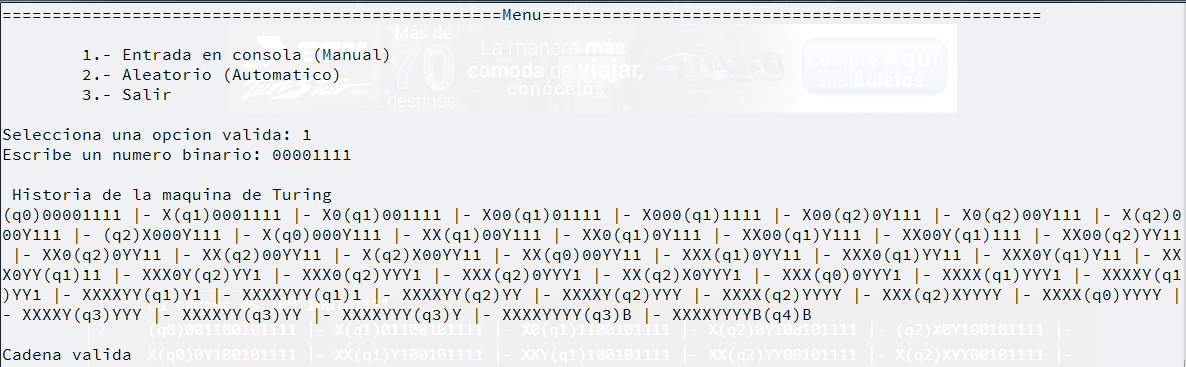
\includegraphics[width=\linewidth, height=7cm]{img/turing-manual-consola.png}
			\caption{Parte de la historia de la Maquina de Turing en consola.}
			\label{fig:turing1}
		\end{center}
	\end{figure}
	\begin{figure}[H]
		\begin{center}
			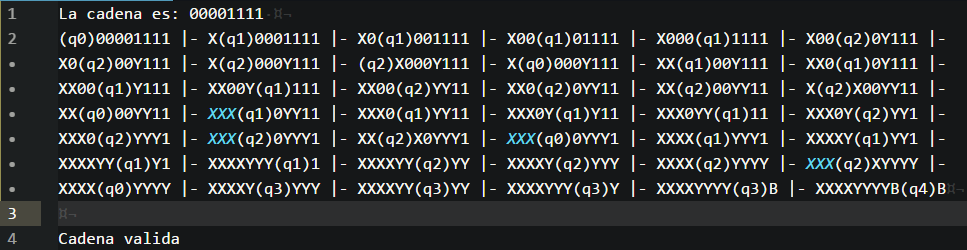
\includegraphics[width=\linewidth, height=5cm]{img/turing-manual-archivo.png}
			\caption{Historia de la Maquina de Turing en archivo.}
			\label{fig:turing2}
		\end{center}
	\end{figure}
	\newpage
	{\large Modo automático}
	\begin{figure}[H]
		\begin{center}
			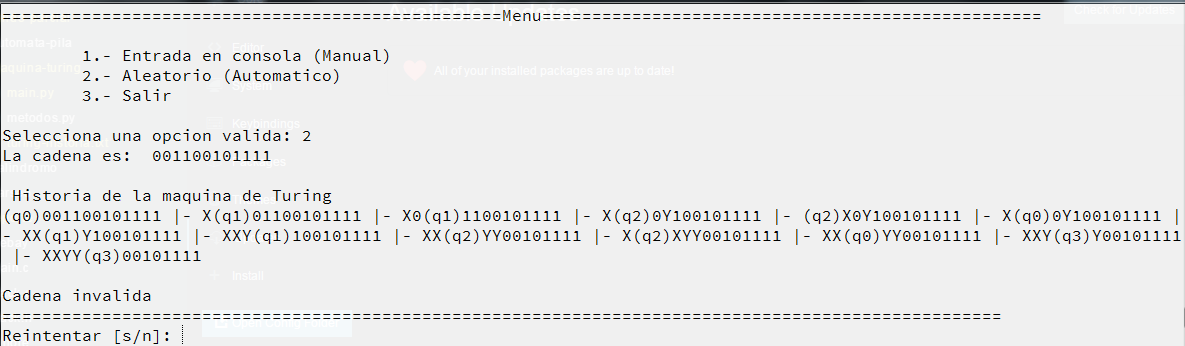
\includegraphics[width=\linewidth, height=7cm]{img/turing-automatico-consola.png}
			\caption{Parte de la historia de la Maquina de Turing en consola.}
			\label{fig:turing3}
		\end{center}
	\end{figure}
	\begin{figure}[H]
		\begin{center}
			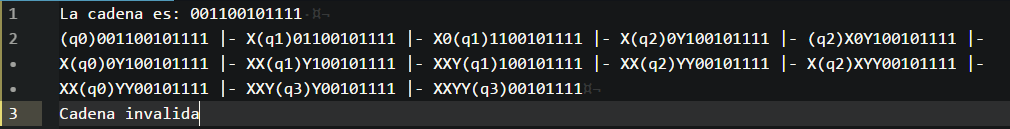
\includegraphics[width=\linewidth, height=4cm]{img/turing-automatico-archivo.png}
			\caption{Historia de la Maquina de Turing en un archivo.}
			\label{fig:turing4}
		\end{center}
	\end{figure}
